\documentclass{article}

\usepackage{graphicx}

\begin{document}

\section*{March 15}
Weather: Sunny turning into overcast, followed by a light drizzle and rain past sunset.

Cleared north bed of the pole bean ``mulch'' by placing the ``mulch'' in the compost. Trying to use pole beans to mulch was a \textit{bad} idea, as all it did was create a slug paradise.

Planted the Southern Row of Peas. Used 3 cups of TCF (Territorial's Complete Fetilizer) spread amongst the South Row, but tilled the whole bed. Sowed Peas approximately 1.5 inches deep, attempting ``several seeds per inch'', but probably ended up a bit short.

\begin{figure}
\protect 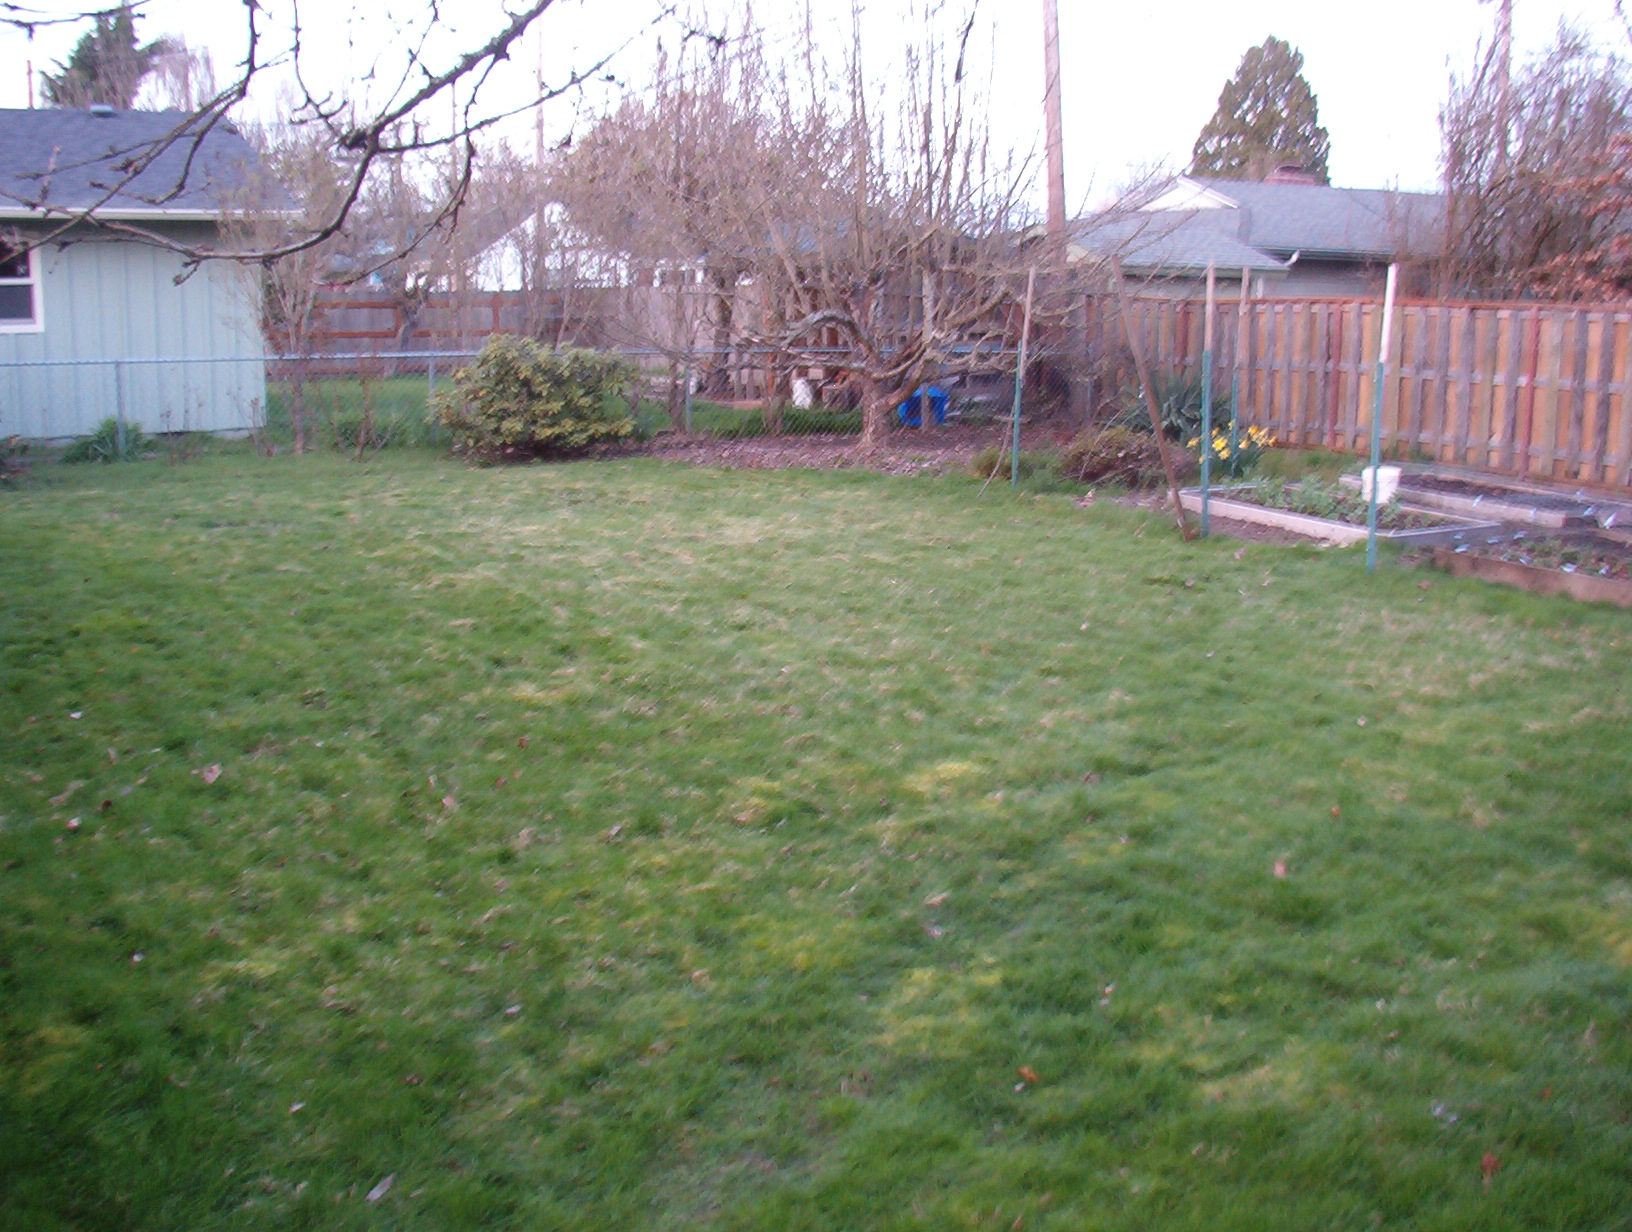
\includegraphics[scale=0.20]{pics/0315_garden1.jpg}
\caption{Weekly north-facing picture of the garden.}
\end{figure}
\begin{figure}
\protect 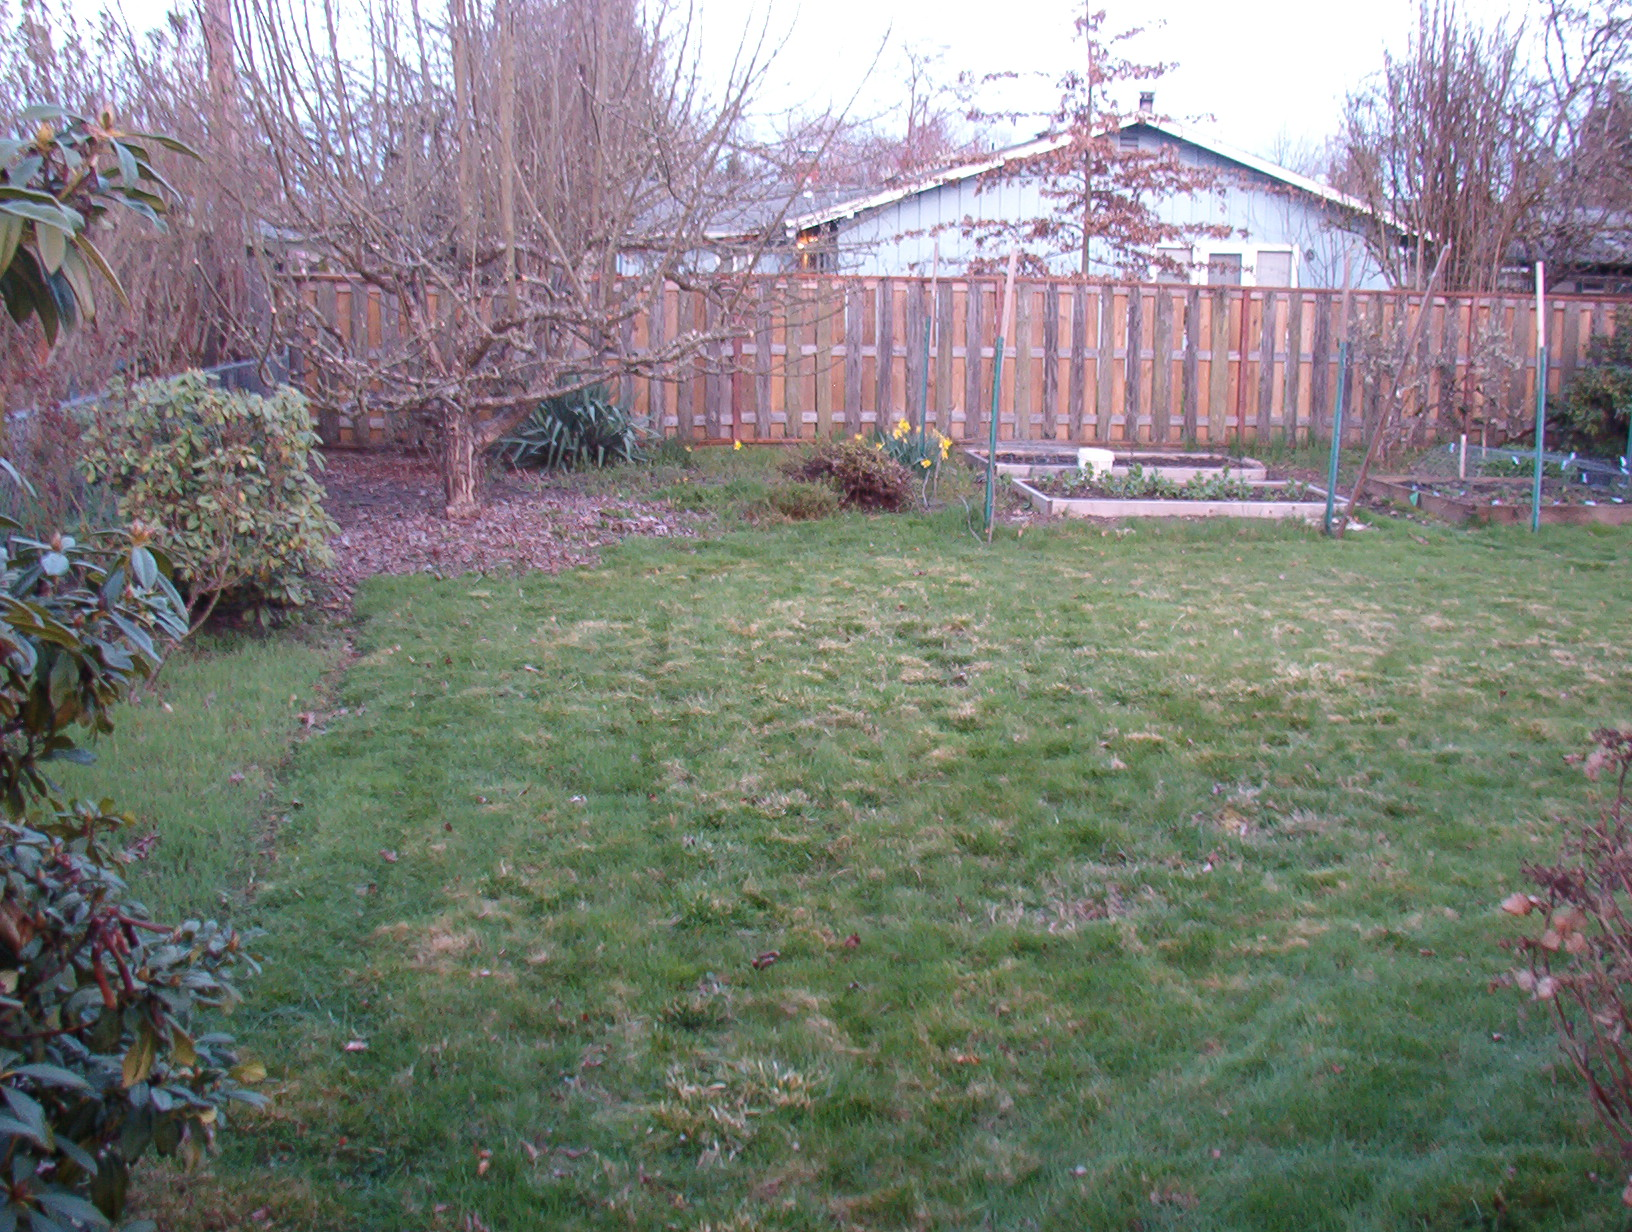
\includegraphics[scale=0.20]{pics/0315_garden2.jpg}
\caption{Weekly east-facing picture of the garden.}
\end{figure}

\section*{March 16}
Weather: Overcast, windy, and cold. Very ominous.

Found issue with garden plan that added extra foot to the available area; managed to fix by compressing the path up against the bed (I wasn't planning on walking that path anyways, right?).

Placed posts to showing started and ending locations of each vegetable patch, except for the one next to the raised bed, since a bush in the way of the final ending point.

\section*{March 17}
Weather: Sunny with a few clouds.

Prepared the Spinach bed. Since the area was already covered by grass, I shoveled the grass off to one side then dug a bit deeper and shoveled the deeper subsoil to another side; I then put the grass back into the bed followed by the deeper subsoil; this may or may not work, because the top and subsoil are horrendous clay. I then tilled 2 cups of TCF into the top 6 row-feet of the bed and attempted to plant about 3 seeds per inch, but probably planted quite a bit more than that (see Figure \ref{0317sowingspinach}) \\
\begin{figure}
\protect 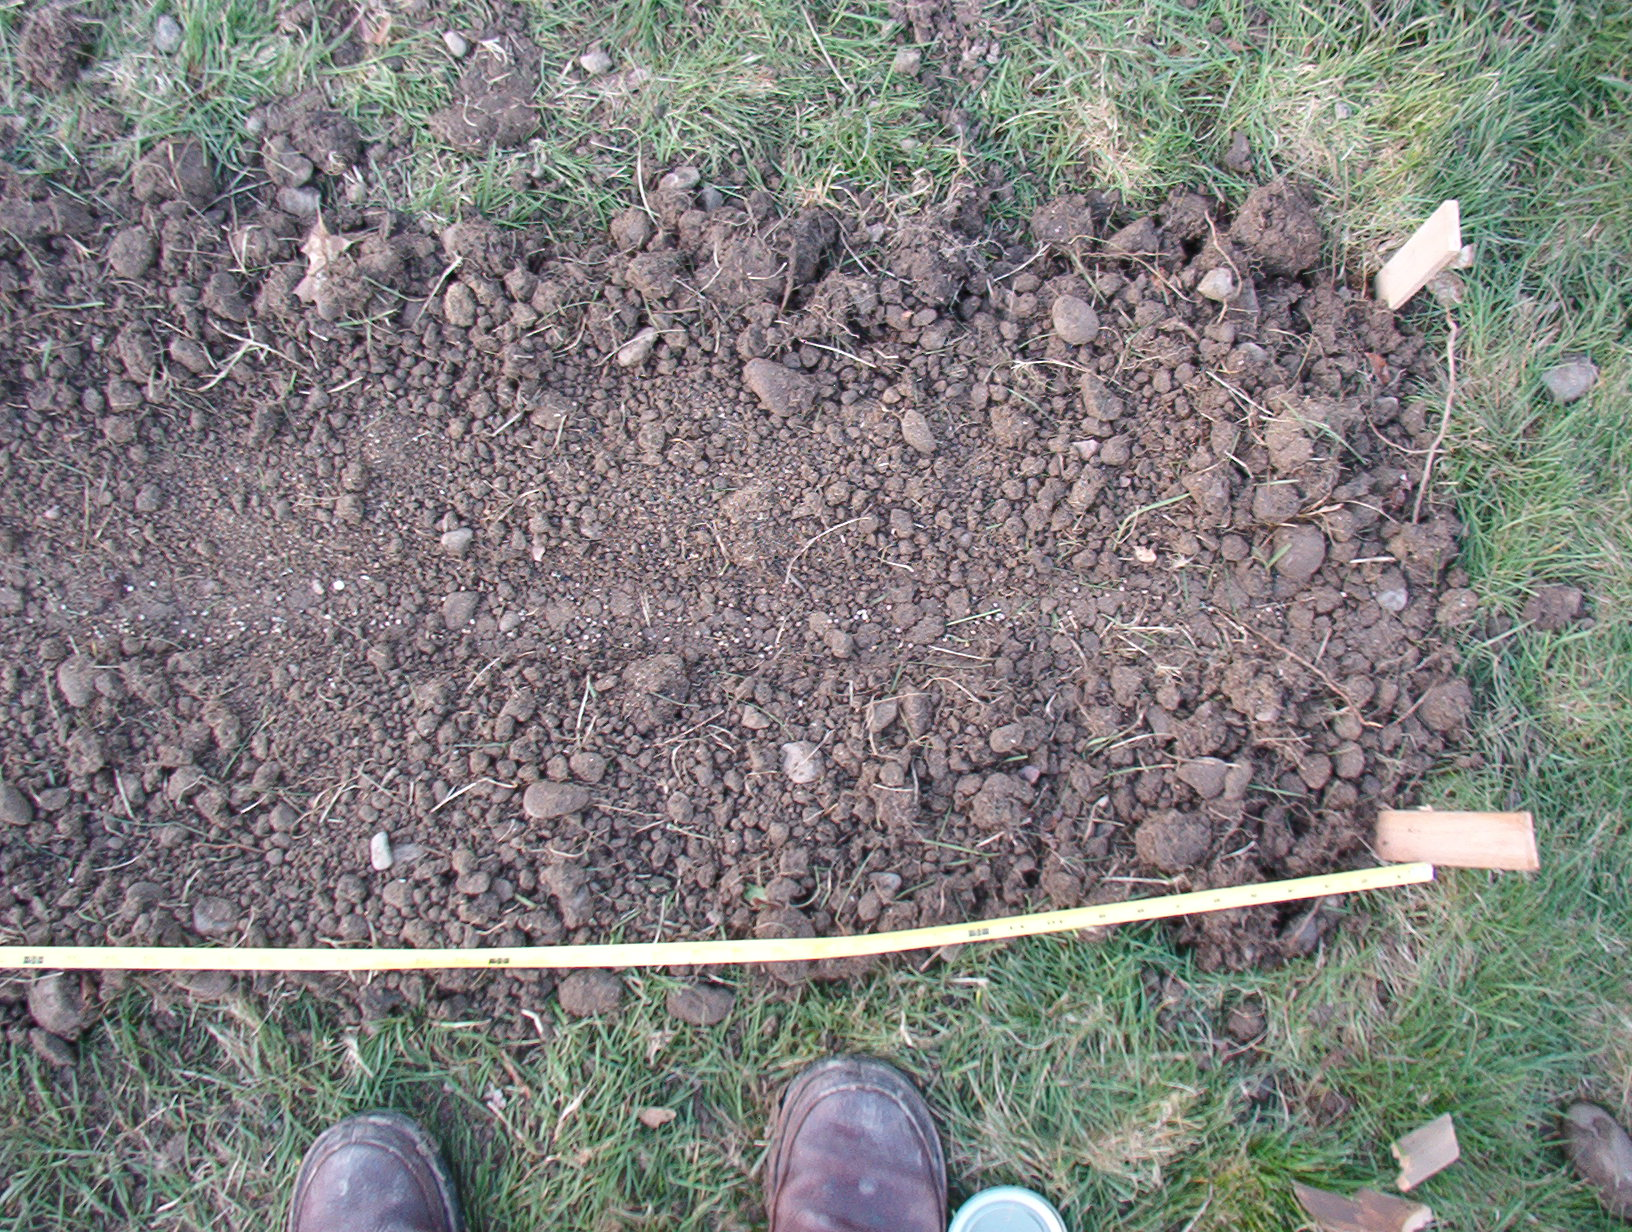
\includegraphics[scale=0.20]{pics/0317_spinach1.jpg}
\protect 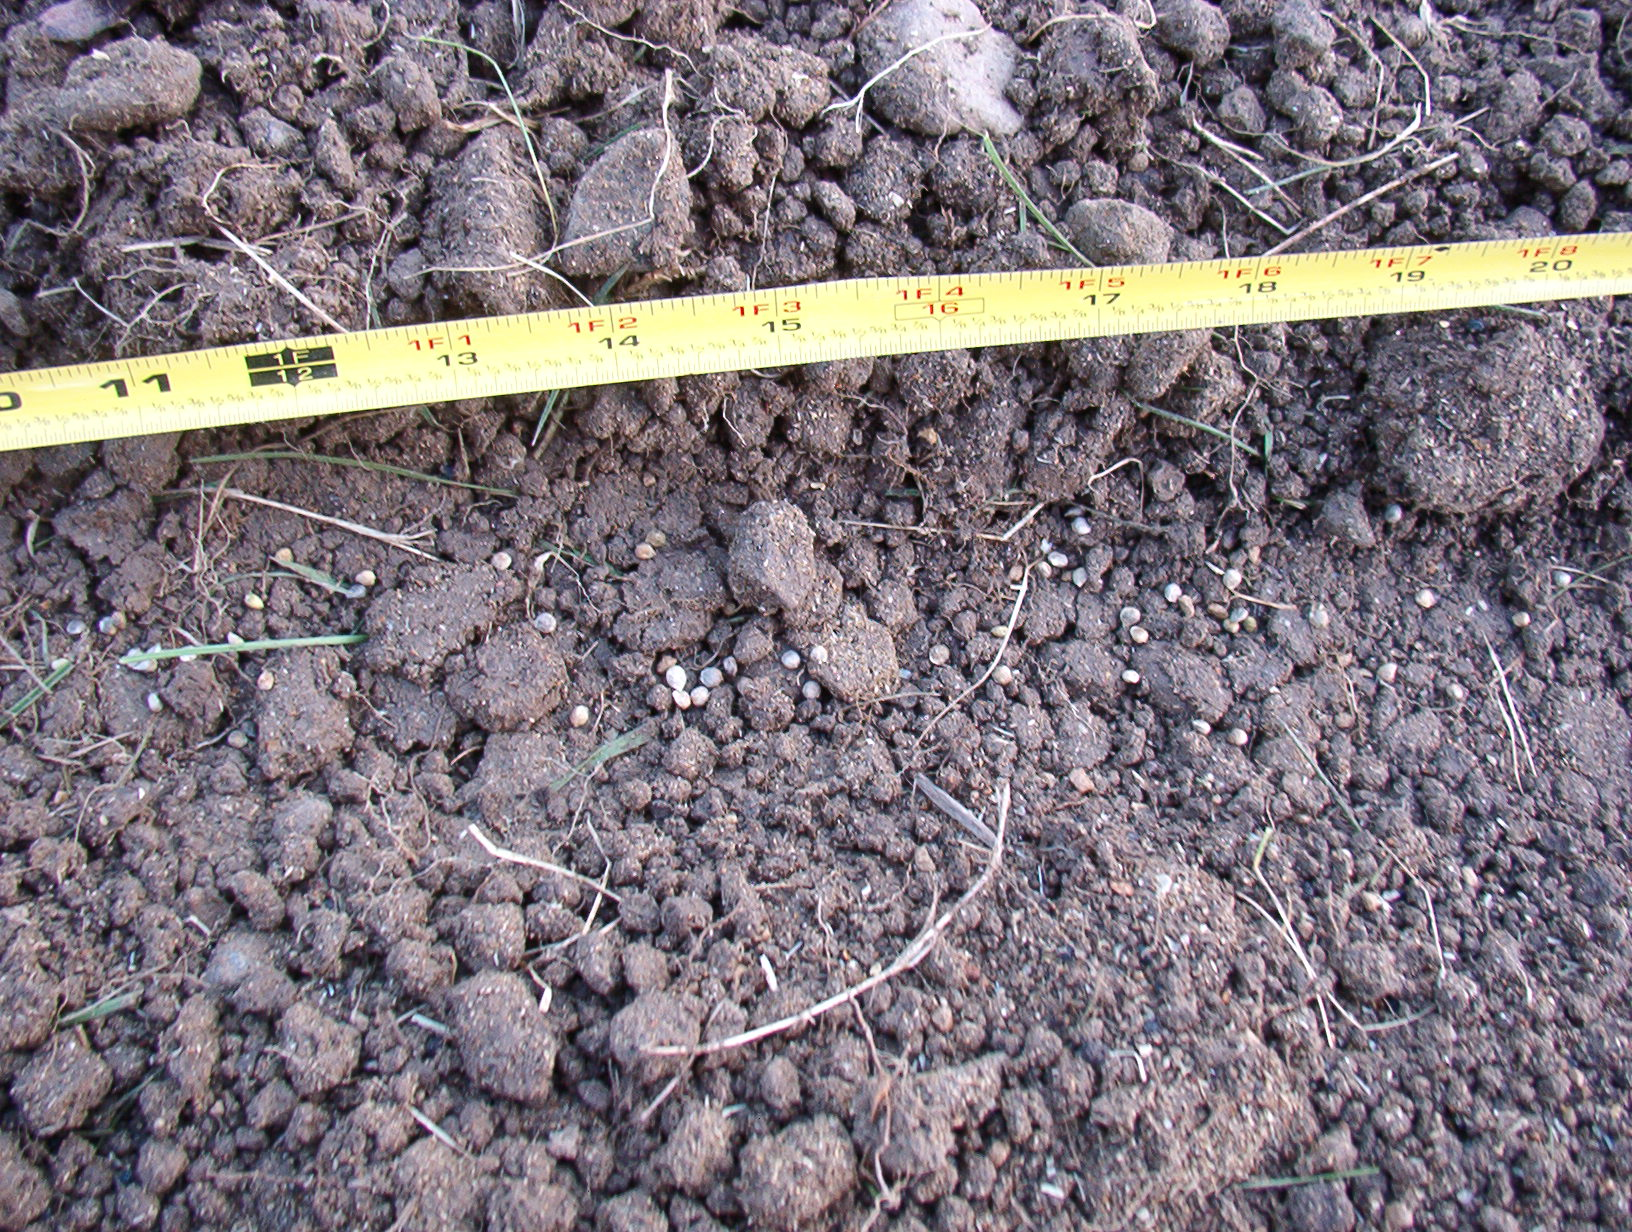
\includegraphics[scale=0.20]{pics/0317_spinach2.jpg}
\caption{Sowing spinach seeds.}
\label{0317sowingspinach}
\end{figure}
That should be okay, since I expect heavy losses. I also expect to side-dress abundantly once (perhaps ``if'') the Spinach germinates. Sown approximately 0.5 inches deep. May need to buy more Spinach needs. I'd like to cover the grass around the bed with paper in order to kill the grass, too, before it starts trying to take over the bed. \\
\begin{figure}
\protect 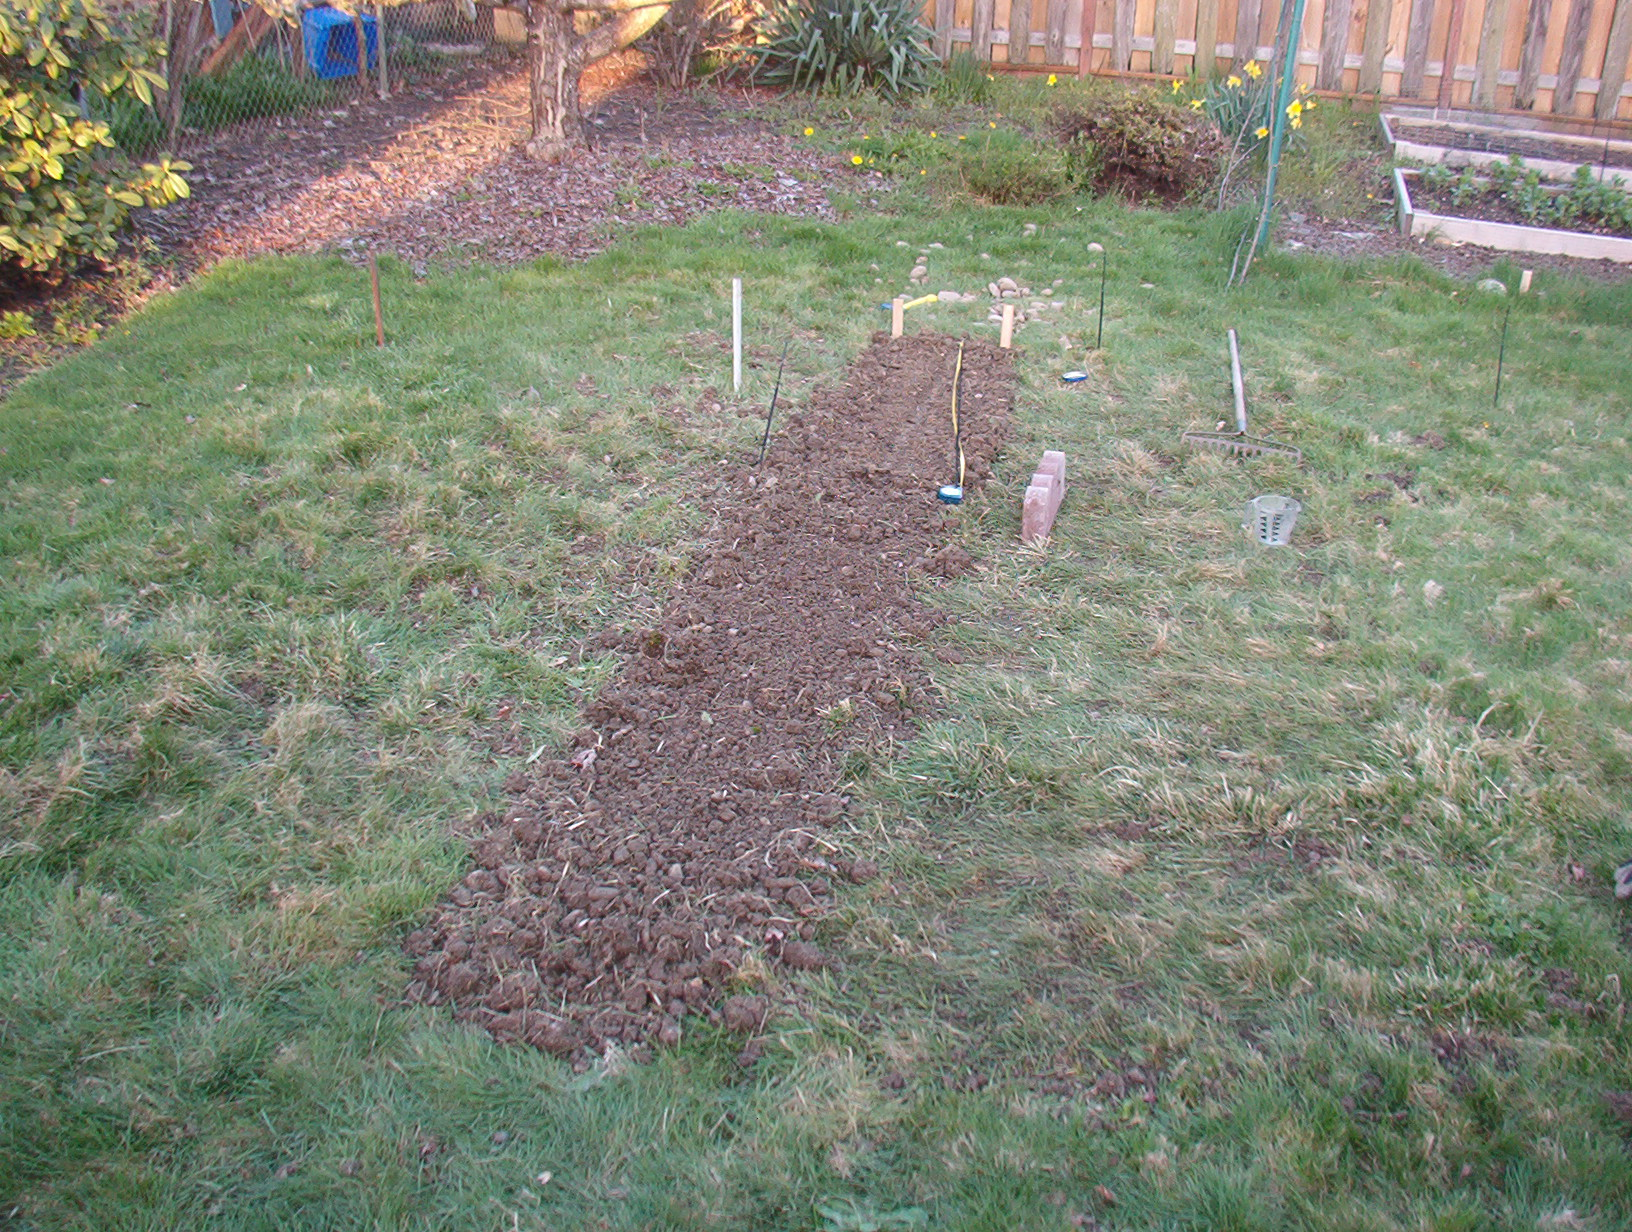
\includegraphics[scale=0.20]{pics/0317_bed.jpg}
\caption{Spinach bed after sowing.}
\end{figure}

\end{document}
